\documentclass[12pt]{article}
\usepackage[letterpaper, top=0.7in, bottom=0.75in, left=0.7in, right=0.7in,
  headheight=15pt, headsep=12pt, footskip=26pt]{geometry}
\usepackage[T1]{fontenc}
\usepackage{helvet}
\renewcommand{\familydefault}{\sfdefault}
\usepackage{tikz}
\usetikzlibrary{arrows.meta}
\usepackage{fancyhdr}
\pagestyle{fancy}
\fancyhf{}
\lhead{Week 63 / Cards away from home / K--1}
\lfoot{Bellingham Math Circle / Week 63 / W63-RV-K-v1}
\rfoot{\thepage}
\renewcommand{\headrulewidth}{0.4pt}
\setlength{\parindent}{0pt}
\setlength{\parskip}{0pt}
\newcommand{\prob}[1]{\textbf{Problem #1:}}
\begin{document}
The homes stay in place. A card is at home when it sits under its own letter and picture. A swap trades the places of any two cards, near or far. Write each swap as the letters of the two cards it trades.

\vspace{2mm}

\par\vspace{3mm}\noindent\hspace*{20mm}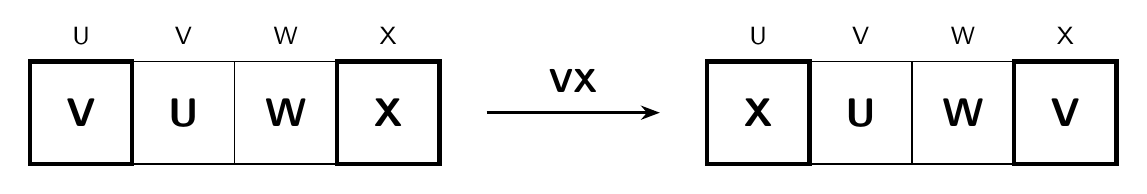
\begin{tikzpicture}[x=1mm, y=1mm]
\draw[line width=1.6pt] (0,0) rectangle (13,13);
\node[inner sep=0, font=\fontsize{9}{10.8}\selectfont] at (6.5,16.2) {U};
\node[inner sep=0, font=\fontsize{15}{18.0}\selectfont\bfseries] at (6.5,6.5) {V};
\draw[line width=0.6pt] (13,0) rectangle (26,13);
\node[inner sep=0, font=\fontsize{9}{10.8}\selectfont] at (19.5,16.2) {V};
\node[inner sep=0, font=\fontsize{15}{18.0}\selectfont\bfseries] at (19.5,6.5) {U};
\draw[line width=0.6pt] (26,0) rectangle (39,13);
\node[inner sep=0, font=\fontsize{9}{10.8}\selectfont] at (32.5,16.2) {W};
\node[inner sep=0, font=\fontsize{15}{18.0}\selectfont\bfseries] at (32.5,6.5) {W};
\draw[line width=1.6pt] (39,0) rectangle (52,13);
\node[inner sep=0, font=\fontsize{9}{10.8}\selectfont] at (45.5,16.2) {X};
\node[inner sep=0, font=\fontsize{15}{18.0}\selectfont\bfseries] at (45.5,6.5) {X};
\draw[-{Stealth[length=2.4mm]}, line width=0.9pt] (58,6.5) -- (80,6.5);
\node[font=\fontsize{12}{14.4}\selectfont\bfseries] at (69,10.5) {VX};
\draw[line width=1.6pt] (86,0) rectangle (99,13);
\node[inner sep=0, font=\fontsize{9}{10.8}\selectfont] at (92.5,16.2) {U};
\node[inner sep=0, font=\fontsize{15}{18.0}\selectfont\bfseries] at (92.5,6.5) {X};
\draw[line width=0.6pt] (99,0) rectangle (112,13);
\node[inner sep=0, font=\fontsize{9}{10.8}\selectfont] at (105.5,16.2) {V};
\node[inner sep=0, font=\fontsize{15}{18.0}\selectfont\bfseries] at (105.5,6.5) {U};
\draw[line width=0.6pt] (112,0) rectangle (125,13);
\node[inner sep=0, font=\fontsize{9}{10.8}\selectfont] at (118.5,16.2) {W};
\node[inner sep=0, font=\fontsize{15}{18.0}\selectfont\bfseries] at (118.5,6.5) {W};
\draw[line width=1.6pt] (125,0) rectangle (138,13);
\node[inner sep=0, font=\fontsize{9}{10.8}\selectfont] at (131.5,16.2) {X};
\node[inner sep=0, font=\fontsize{15}{18.0}\selectfont\bfseries] at (131.5,6.5) {V};
\end{tikzpicture}\par

\vspace{9mm}
\prob{1} Start with A, B and C at home. Swap cards until no card is at home, using as few swaps as you can.

\par\vspace{3mm}\noindent\hspace*{2mm}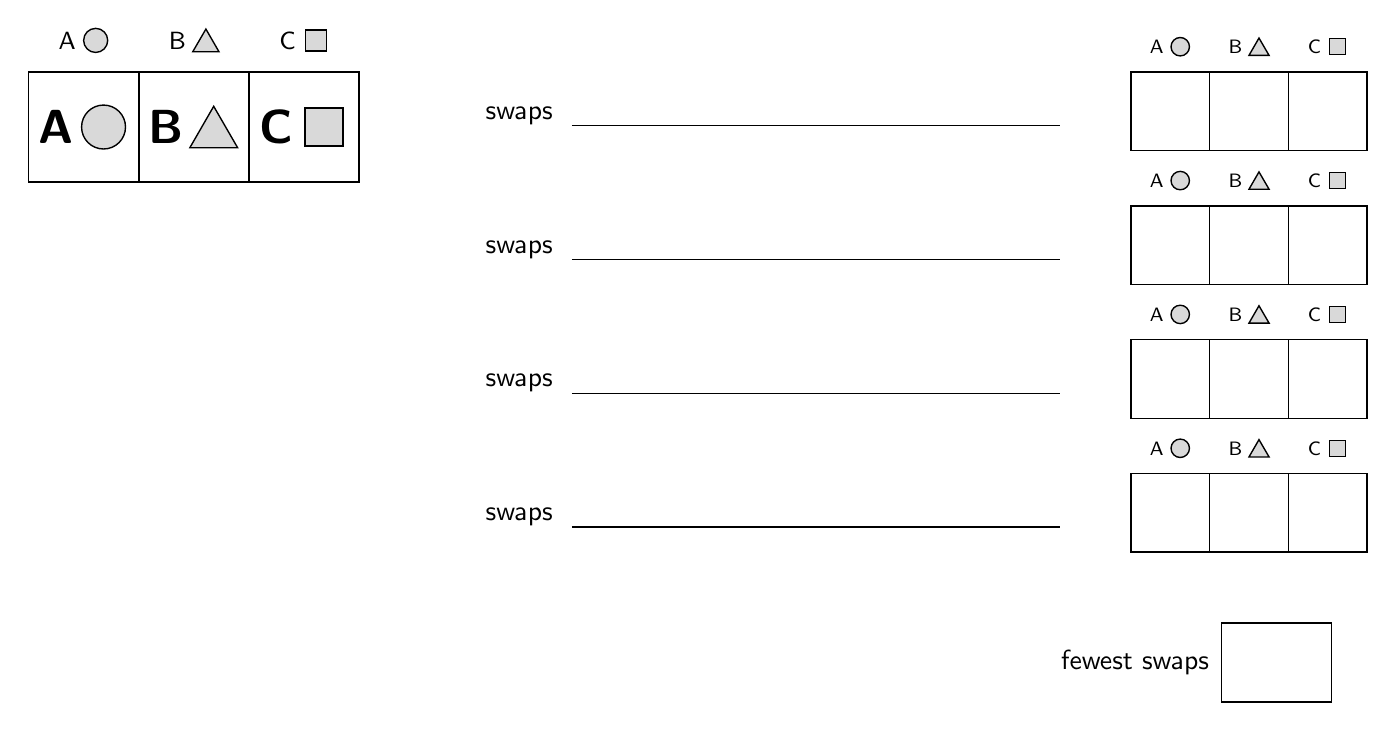
\begin{tikzpicture}[x=1mm, y=1mm]
\draw[line width=0.6pt] (0,0) rectangle (14,14);
\node[inner sep=0, font=\fontsize{9}{10.8}\selectfont] at (4.9,18) {A};
\path[fill=gray!30, draw=black, line width=0.5pt] (8.53,18) circle (1.53);
\node[inner sep=0, font=\fontsize{17}{20.4}\selectfont\bfseries] at (3.5,7) {A};
\path[fill=gray!30, draw=black, line width=0.5pt] (9.53,7) circle (2.79);
\draw[line width=0.6pt] (14,0) rectangle (28,14);
\node[inner sep=0, font=\fontsize{9}{10.8}\selectfont] at (18.9,18) {B};
\path[fill=gray!30, draw=black, line width=0.5pt] (22.53,19.44) -- (20.86,16.56) -- (24.19,16.56) -- cycle;
\node[inner sep=0, font=\fontsize{17}{20.4}\selectfont\bfseries] at (17.5,7) {B};
\path[fill=gray!30, draw=black, line width=0.5pt] (23.52,9.63) -- (20.49,4.37) -- (26.56,4.37) -- cycle;
\draw[line width=0.6pt] (28,0) rectangle (42,14);
\node[inner sep=0, font=\fontsize{9}{10.8}\selectfont] at (32.9,18) {C};
\path[fill=gray!30, draw=black, line width=0.5pt] (35.2,16.67) rectangle (37.85,19.33);
\node[inner sep=0, font=\fontsize{17}{20.4}\selectfont\bfseries] at (31.5,7) {C};
\path[fill=gray!30, draw=black, line width=0.5pt] (35.11,4.58) rectangle (39.94,9.42);
\node[anchor=base west, inner sep=0, font=\fontsize{10}{12.0}\selectfont] at (58,8) {swaps};
\draw[line width=0.4pt] (69,7.2) -- (131,7.2);
\draw[line width=0.6pt] (140,4) rectangle (150,14);
\node[inner sep=0, font=\fontsize{7}{8.4}\selectfont] at (143.3,17.2) {A};
\path[fill=gray!30, draw=black, line width=0.5pt] (146.27,17.2) circle (1.17);
\draw[line width=0.6pt] (150,4) rectangle (160,14);
\node[inner sep=0, font=\fontsize{7}{8.4}\selectfont] at (153.3,17.2) {B};
\path[fill=gray!30, draw=black, line width=0.5pt] (156.27,18.3) -- (155,16.1) -- (157.55,16.1) -- cycle;
\draw[line width=0.6pt] (160,4) rectangle (170,14);
\node[inner sep=0, font=\fontsize{7}{8.4}\selectfont] at (163.3,17.2) {C};
\path[fill=gray!30, draw=black, line width=0.5pt] (165.26,16.19) rectangle (167.29,18.21);
\node[anchor=base west, inner sep=0, font=\fontsize{10}{12.0}\selectfont] at (58,-9) {swaps};
\draw[line width=0.4pt] (69,-9.8) -- (131,-9.8);
\draw[line width=0.6pt] (140,-13) rectangle (150,-3);
\node[inner sep=0, font=\fontsize{7}{8.4}\selectfont] at (143.3,0.2) {A};
\path[fill=gray!30, draw=black, line width=0.5pt] (146.27,0.2) circle (1.17);
\draw[line width=0.6pt] (150,-13) rectangle (160,-3);
\node[inner sep=0, font=\fontsize{7}{8.4}\selectfont] at (153.3,0.2) {B};
\path[fill=gray!30, draw=black, line width=0.5pt] (156.27,1.3) -- (155,-0.9) -- (157.55,-0.9) -- cycle;
\draw[line width=0.6pt] (160,-13) rectangle (170,-3);
\node[inner sep=0, font=\fontsize{7}{8.4}\selectfont] at (163.3,0.2) {C};
\path[fill=gray!30, draw=black, line width=0.5pt] (165.26,-0.81) rectangle (167.29,1.21);
\node[anchor=base west, inner sep=0, font=\fontsize{10}{12.0}\selectfont] at (58,-26) {swaps};
\draw[line width=0.4pt] (69,-26.8) -- (131,-26.8);
\draw[line width=0.6pt] (140,-30) rectangle (150,-20);
\node[inner sep=0, font=\fontsize{7}{8.4}\selectfont] at (143.3,-16.8) {A};
\path[fill=gray!30, draw=black, line width=0.5pt] (146.27,-16.8) circle (1.17);
\draw[line width=0.6pt] (150,-30) rectangle (160,-20);
\node[inner sep=0, font=\fontsize{7}{8.4}\selectfont] at (153.3,-16.8) {B};
\path[fill=gray!30, draw=black, line width=0.5pt] (156.27,-15.7) -- (155,-17.9) -- (157.55,-17.9) -- cycle;
\draw[line width=0.6pt] (160,-30) rectangle (170,-20);
\node[inner sep=0, font=\fontsize{7}{8.4}\selectfont] at (163.3,-16.8) {C};
\path[fill=gray!30, draw=black, line width=0.5pt] (165.26,-17.81) rectangle (167.29,-15.79);
\node[anchor=base west, inner sep=0, font=\fontsize{10}{12.0}\selectfont] at (58,-43) {swaps};
\draw[line width=0.4pt] (69,-43.8) -- (131,-43.8);
\draw[line width=0.6pt] (140,-47) rectangle (150,-37);
\node[inner sep=0, font=\fontsize{7}{8.4}\selectfont] at (143.3,-33.8) {A};
\path[fill=gray!30, draw=black, line width=0.5pt] (146.27,-33.8) circle (1.17);
\draw[line width=0.6pt] (150,-47) rectangle (160,-37);
\node[inner sep=0, font=\fontsize{7}{8.4}\selectfont] at (153.3,-33.8) {B};
\path[fill=gray!30, draw=black, line width=0.5pt] (156.27,-32.7) -- (155,-34.9) -- (157.55,-34.9) -- cycle;
\draw[line width=0.6pt] (160,-47) rectangle (170,-37);
\node[inner sep=0, font=\fontsize{7}{8.4}\selectfont] at (163.3,-33.8) {C};
\path[fill=gray!30, draw=black, line width=0.5pt] (165.26,-34.81) rectangle (167.29,-32.79);
\node[anchor=east, inner sep=0, font=\fontsize{10}{12.0}\selectfont] at (150,-61) {fewest swaps};
\draw[line width=0.6pt] (151.5,-66) rectangle (165.5,-56);
\end{tikzpicture}\par

\newpage
\prob{2} Do Problem 1 again with A, B, C and D. Which rows can you end with in the fewest swaps?

\par\vspace{3mm}\noindent\hspace*{2mm}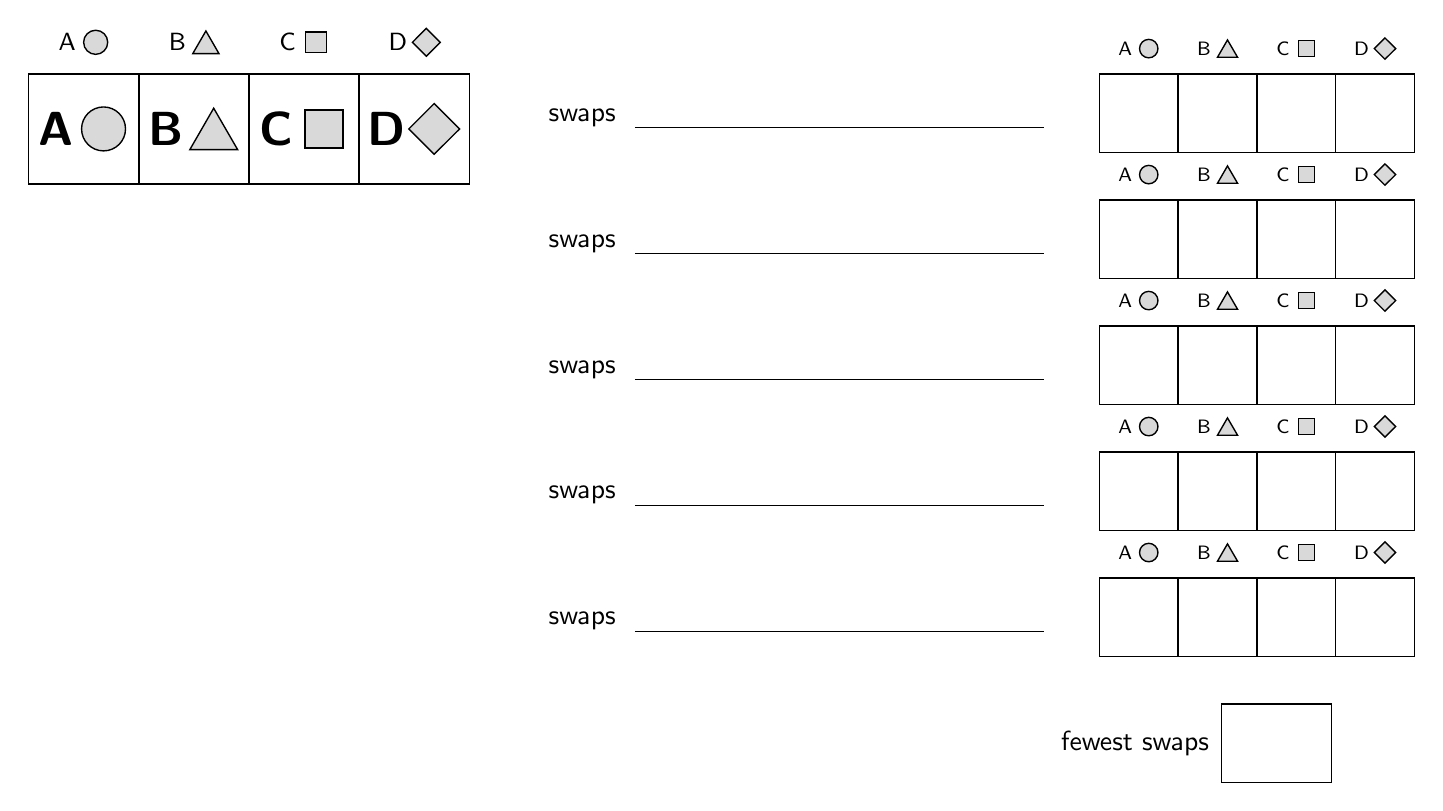
\begin{tikzpicture}[x=1mm, y=1mm]
\draw[line width=0.6pt] (0,0) rectangle (14,14);
\node[inner sep=0, font=\fontsize{9}{10.8}\selectfont] at (4.9,18) {A};
\path[fill=gray!30, draw=black, line width=0.5pt] (8.53,18) circle (1.53);
\node[inner sep=0, font=\fontsize{17}{20.4}\selectfont\bfseries] at (3.5,7) {A};
\path[fill=gray!30, draw=black, line width=0.5pt] (9.53,7) circle (2.79);
\draw[line width=0.6pt] (14,0) rectangle (28,14);
\node[inner sep=0, font=\fontsize{9}{10.8}\selectfont] at (18.9,18) {B};
\path[fill=gray!30, draw=black, line width=0.5pt] (22.53,19.44) -- (20.86,16.56) -- (24.19,16.56) -- cycle;
\node[inner sep=0, font=\fontsize{17}{20.4}\selectfont\bfseries] at (17.5,7) {B};
\path[fill=gray!30, draw=black, line width=0.5pt] (23.52,9.63) -- (20.49,4.37) -- (26.56,4.37) -- cycle;
\draw[line width=0.6pt] (28,0) rectangle (42,14);
\node[inner sep=0, font=\fontsize{9}{10.8}\selectfont] at (32.9,18) {C};
\path[fill=gray!30, draw=black, line width=0.5pt] (35.2,16.67) rectangle (37.85,19.33);
\node[inner sep=0, font=\fontsize{17}{20.4}\selectfont\bfseries] at (31.5,7) {C};
\path[fill=gray!30, draw=black, line width=0.5pt] (35.11,4.58) rectangle (39.94,9.42);
\draw[line width=0.6pt] (42,0) rectangle (56,14);
\node[inner sep=0, font=\fontsize{9}{10.8}\selectfont] at (46.9,18) {D};
\path[fill=gray!30, draw=black, line width=0.5pt] (50.52,19.77) -- (52.29,18) -- (50.52,16.23) -- (48.76,18) -- cycle;
\node[inner sep=0, font=\fontsize{17}{20.4}\selectfont\bfseries] at (45.5,7) {D};
\path[fill=gray!30, draw=black, line width=0.5pt] (51.52,10.22) -- (54.75,7) -- (51.52,3.78) -- (48.3,7) -- cycle;
\node[anchor=base west, inner sep=0, font=\fontsize{10}{12.0}\selectfont] at (66,8) {swaps};
\draw[line width=0.4pt] (77,7.2) -- (129,7.2);
\draw[line width=0.6pt] (136,4) rectangle (146,14);
\node[inner sep=0, font=\fontsize{7}{8.4}\selectfont] at (139.3,17.2) {A};
\path[fill=gray!30, draw=black, line width=0.5pt] (142.27,17.2) circle (1.17);
\draw[line width=0.6pt] (146,4) rectangle (156,14);
\node[inner sep=0, font=\fontsize{7}{8.4}\selectfont] at (149.3,17.2) {B};
\path[fill=gray!30, draw=black, line width=0.5pt] (152.27,18.3) -- (151,16.1) -- (153.55,16.1) -- cycle;
\draw[line width=0.6pt] (156,4) rectangle (166,14);
\node[inner sep=0, font=\fontsize{7}{8.4}\selectfont] at (159.3,17.2) {C};
\path[fill=gray!30, draw=black, line width=0.5pt] (161.26,16.19) rectangle (163.29,18.21);
\draw[line width=0.6pt] (166,4) rectangle (176,14);
\node[inner sep=0, font=\fontsize{7}{8.4}\selectfont] at (169.3,17.2) {D};
\path[fill=gray!30, draw=black, line width=0.5pt] (172.27,18.55) -- (173.63,17.2) -- (172.27,15.85) -- (170.92,17.2) -- cycle;
\node[anchor=base west, inner sep=0, font=\fontsize{10}{12.0}\selectfont] at (66,-8) {swaps};
\draw[line width=0.4pt] (77,-8.8) -- (129,-8.8);
\draw[line width=0.6pt] (136,-12) rectangle (146,-2);
\node[inner sep=0, font=\fontsize{7}{8.4}\selectfont] at (139.3,1.2) {A};
\path[fill=gray!30, draw=black, line width=0.5pt] (142.27,1.2) circle (1.17);
\draw[line width=0.6pt] (146,-12) rectangle (156,-2);
\node[inner sep=0, font=\fontsize{7}{8.4}\selectfont] at (149.3,1.2) {B};
\path[fill=gray!30, draw=black, line width=0.5pt] (152.27,2.3) -- (151,0.1) -- (153.55,0.1) -- cycle;
\draw[line width=0.6pt] (156,-12) rectangle (166,-2);
\node[inner sep=0, font=\fontsize{7}{8.4}\selectfont] at (159.3,1.2) {C};
\path[fill=gray!30, draw=black, line width=0.5pt] (161.26,0.19) rectangle (163.29,2.21);
\draw[line width=0.6pt] (166,-12) rectangle (176,-2);
\node[inner sep=0, font=\fontsize{7}{8.4}\selectfont] at (169.3,1.2) {D};
\path[fill=gray!30, draw=black, line width=0.5pt] (172.27,2.55) -- (173.63,1.2) -- (172.27,-0.15) -- (170.92,1.2) -- cycle;
\node[anchor=base west, inner sep=0, font=\fontsize{10}{12.0}\selectfont] at (66,-24) {swaps};
\draw[line width=0.4pt] (77,-24.8) -- (129,-24.8);
\draw[line width=0.6pt] (136,-28) rectangle (146,-18);
\node[inner sep=0, font=\fontsize{7}{8.4}\selectfont] at (139.3,-14.8) {A};
\path[fill=gray!30, draw=black, line width=0.5pt] (142.27,-14.8) circle (1.17);
\draw[line width=0.6pt] (146,-28) rectangle (156,-18);
\node[inner sep=0, font=\fontsize{7}{8.4}\selectfont] at (149.3,-14.8) {B};
\path[fill=gray!30, draw=black, line width=0.5pt] (152.27,-13.7) -- (151,-15.9) -- (153.55,-15.9) -- cycle;
\draw[line width=0.6pt] (156,-28) rectangle (166,-18);
\node[inner sep=0, font=\fontsize{7}{8.4}\selectfont] at (159.3,-14.8) {C};
\path[fill=gray!30, draw=black, line width=0.5pt] (161.26,-15.81) rectangle (163.29,-13.79);
\draw[line width=0.6pt] (166,-28) rectangle (176,-18);
\node[inner sep=0, font=\fontsize{7}{8.4}\selectfont] at (169.3,-14.8) {D};
\path[fill=gray!30, draw=black, line width=0.5pt] (172.27,-13.45) -- (173.63,-14.8) -- (172.27,-16.15) -- (170.92,-14.8) -- cycle;
\node[anchor=base west, inner sep=0, font=\fontsize{10}{12.0}\selectfont] at (66,-40) {swaps};
\draw[line width=0.4pt] (77,-40.8) -- (129,-40.8);
\draw[line width=0.6pt] (136,-44) rectangle (146,-34);
\node[inner sep=0, font=\fontsize{7}{8.4}\selectfont] at (139.3,-30.8) {A};
\path[fill=gray!30, draw=black, line width=0.5pt] (142.27,-30.8) circle (1.17);
\draw[line width=0.6pt] (146,-44) rectangle (156,-34);
\node[inner sep=0, font=\fontsize{7}{8.4}\selectfont] at (149.3,-30.8) {B};
\path[fill=gray!30, draw=black, line width=0.5pt] (152.27,-29.7) -- (151,-31.9) -- (153.55,-31.9) -- cycle;
\draw[line width=0.6pt] (156,-44) rectangle (166,-34);
\node[inner sep=0, font=\fontsize{7}{8.4}\selectfont] at (159.3,-30.8) {C};
\path[fill=gray!30, draw=black, line width=0.5pt] (161.26,-31.81) rectangle (163.29,-29.79);
\draw[line width=0.6pt] (166,-44) rectangle (176,-34);
\node[inner sep=0, font=\fontsize{7}{8.4}\selectfont] at (169.3,-30.8) {D};
\path[fill=gray!30, draw=black, line width=0.5pt] (172.27,-29.45) -- (173.63,-30.8) -- (172.27,-32.15) -- (170.92,-30.8) -- cycle;
\node[anchor=base west, inner sep=0, font=\fontsize{10}{12.0}\selectfont] at (66,-56) {swaps};
\draw[line width=0.4pt] (77,-56.8) -- (129,-56.8);
\draw[line width=0.6pt] (136,-60) rectangle (146,-50);
\node[inner sep=0, font=\fontsize{7}{8.4}\selectfont] at (139.3,-46.8) {A};
\path[fill=gray!30, draw=black, line width=0.5pt] (142.27,-46.8) circle (1.17);
\draw[line width=0.6pt] (146,-60) rectangle (156,-50);
\node[inner sep=0, font=\fontsize{7}{8.4}\selectfont] at (149.3,-46.8) {B};
\path[fill=gray!30, draw=black, line width=0.5pt] (152.27,-45.7) -- (151,-47.9) -- (153.55,-47.9) -- cycle;
\draw[line width=0.6pt] (156,-60) rectangle (166,-50);
\node[inner sep=0, font=\fontsize{7}{8.4}\selectfont] at (159.3,-46.8) {C};
\path[fill=gray!30, draw=black, line width=0.5pt] (161.26,-47.81) rectangle (163.29,-45.79);
\draw[line width=0.6pt] (166,-60) rectangle (176,-50);
\node[inner sep=0, font=\fontsize{7}{8.4}\selectfont] at (169.3,-46.8) {D};
\path[fill=gray!30, draw=black, line width=0.5pt] (172.27,-45.45) -- (173.63,-46.8) -- (172.27,-48.15) -- (170.92,-46.8) -- cycle;
\node[anchor=east, inner sep=0, font=\fontsize{10}{12.0}\selectfont] at (150,-71) {fewest swaps};
\draw[line width=0.6pt] (151.5,-76) rectangle (165.5,-66);
\end{tikzpicture}\par

\vfill
\prob{3} Start with all five cards at home. Can two swaps leave no card at home? Can three?

\par\vspace{3mm}\noindent\hspace*{2mm}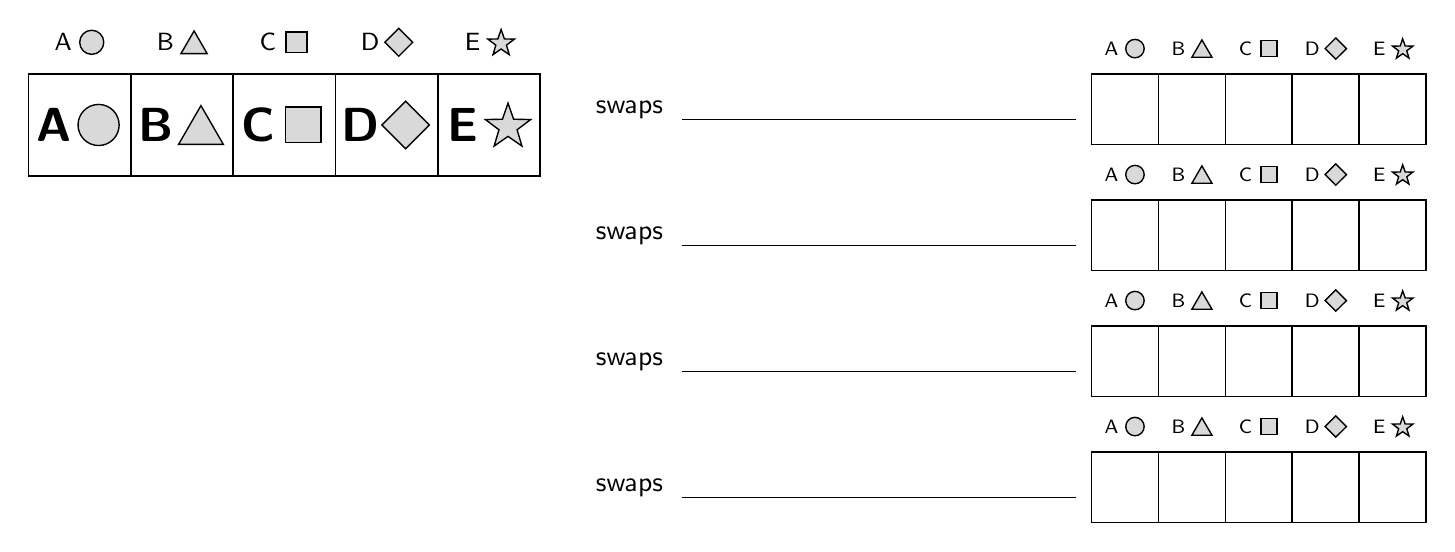
\begin{tikzpicture}[x=1mm, y=1mm]
\draw[line width=0.6pt] (0,0) rectangle (13,13);
\node[inner sep=0, font=\fontsize{9}{10.8}\selectfont] at (4.4,17) {A};
\path[fill=gray!30, draw=black, line width=0.5pt] (8.03,17) circle (1.53);
\node[inner sep=0, font=\fontsize{16}{19.2}\selectfont\bfseries] at (3.2,6.5) {A};
\path[fill=gray!30, draw=black, line width=0.5pt] (8.9,6.5) circle (2.61);
\draw[line width=0.6pt] (13,0) rectangle (26,13);
\node[inner sep=0, font=\fontsize{9}{10.8}\selectfont] at (17.4,17) {B};
\path[fill=gray!30, draw=black, line width=0.5pt] (21.03,18.44) -- (19.36,15.56) -- (22.69,15.56) -- cycle;
\node[inner sep=0, font=\fontsize{16}{19.2}\selectfont\bfseries] at (16.2,6.5) {B};
\path[fill=gray!30, draw=black, line width=0.5pt] (21.9,8.96) -- (19.06,4.04) -- (24.74,4.04) -- cycle;
\draw[line width=0.6pt] (26,0) rectangle (39,13);
\node[inner sep=0, font=\fontsize{9}{10.8}\selectfont] at (30.4,17) {C};
\path[fill=gray!30, draw=black, line width=0.5pt] (32.7,15.67) rectangle (35.35,18.33);
\node[inner sep=0, font=\fontsize{16}{19.2}\selectfont\bfseries] at (29.2,6.5) {C};
\path[fill=gray!30, draw=black, line width=0.5pt] (32.64,4.24) rectangle (37.16,8.76);
\draw[line width=0.6pt] (39,0) rectangle (52,13);
\node[inner sep=0, font=\fontsize{9}{10.8}\selectfont] at (43.4,17) {D};
\path[fill=gray!30, draw=black, line width=0.5pt] (47.02,18.77) -- (48.79,17) -- (47.02,15.23) -- (45.26,17) -- cycle;
\node[inner sep=0, font=\fontsize{16}{19.2}\selectfont\bfseries] at (42.2,6.5) {D};
\path[fill=gray!30, draw=black, line width=0.5pt] (47.9,9.52) -- (50.92,6.5) -- (47.9,3.48) -- (44.88,6.5) -- cycle;
\draw[line width=0.6pt] (52,0) rectangle (65,13);
\node[inner sep=0, font=\fontsize{9}{10.8}\selectfont] at (56.4,17) {E};
\path[fill=gray!30, draw=black, line width=0.5pt] (60.02,18.63) -- (59.61,17.43) -- (58.34,17.4) -- (59.35,16.64) -- (58.99,15.43) -- (60.02,16.15) -- (61.06,15.43) -- (60.7,16.64) -- (61.71,17.4) -- (60.44,17.43) -- cycle;
\node[inner sep=0, font=\fontsize{16}{19.2}\selectfont\bfseries] at (55.2,6.5) {E};
\path[fill=gray!30, draw=black, line width=0.5pt] (60.9,9.27) -- (60.19,7.23) -- (58.03,7.19) -- (59.75,5.89) -- (59.13,3.82) -- (60.9,5.05) -- (62.67,3.82) -- (62.05,5.89) -- (63.77,7.19) -- (61.61,7.23) -- cycle;
\node[anchor=base west, inner sep=0, font=\fontsize{10}{12.0}\selectfont] at (72,8) {swaps};
\draw[line width=0.4pt] (83,7.2) -- (133,7.2);
\draw[line width=0.6pt] (135,4) rectangle (143.5,13);
\node[inner sep=0, font=\fontsize{7}{8.4}\selectfont] at (137.55,16.2) {A};
\path[fill=gray!30, draw=black, line width=0.5pt] (140.52,16.2) circle (1.17);
\draw[line width=0.6pt] (143.5,4) rectangle (152,13);
\node[inner sep=0, font=\fontsize{7}{8.4}\selectfont] at (146.05,16.2) {B};
\path[fill=gray!30, draw=black, line width=0.5pt] (149.02,17.3) -- (147.75,15.1) -- (150.3,15.1) -- cycle;
\draw[line width=0.6pt] (152,4) rectangle (160.5,13);
\node[inner sep=0, font=\fontsize{7}{8.4}\selectfont] at (154.55,16.2) {C};
\path[fill=gray!30, draw=black, line width=0.5pt] (156.51,15.19) rectangle (158.54,17.21);
\draw[line width=0.6pt] (160.5,4) rectangle (169,13);
\node[inner sep=0, font=\fontsize{7}{8.4}\selectfont] at (163.05,16.2) {D};
\path[fill=gray!30, draw=black, line width=0.5pt] (166.02,17.55) -- (167.38,16.2) -- (166.02,14.85) -- (164.67,16.2) -- cycle;
\draw[line width=0.6pt] (169,4) rectangle (177.5,13);
\node[inner sep=0, font=\fontsize{7}{8.4}\selectfont] at (171.55,16.2) {E};
\path[fill=gray!30, draw=black, line width=0.5pt] (174.52,17.44) -- (174.21,16.53) -- (173.24,16.51) -- (174.01,15.92) -- (173.73,15) -- (174.52,15.55) -- (175.32,15) -- (175.04,15.92) -- (175.81,16.51) -- (174.84,16.53) -- cycle;
\node[anchor=base west, inner sep=0, font=\fontsize{10}{12.0}\selectfont] at (72,-8) {swaps};
\draw[line width=0.4pt] (83,-8.8) -- (133,-8.8);
\draw[line width=0.6pt] (135,-12) rectangle (143.5,-3);
\node[inner sep=0, font=\fontsize{7}{8.4}\selectfont] at (137.55,0.2) {A};
\path[fill=gray!30, draw=black, line width=0.5pt] (140.52,0.2) circle (1.17);
\draw[line width=0.6pt] (143.5,-12) rectangle (152,-3);
\node[inner sep=0, font=\fontsize{7}{8.4}\selectfont] at (146.05,0.2) {B};
\path[fill=gray!30, draw=black, line width=0.5pt] (149.02,1.3) -- (147.75,-0.9) -- (150.3,-0.9) -- cycle;
\draw[line width=0.6pt] (152,-12) rectangle (160.5,-3);
\node[inner sep=0, font=\fontsize{7}{8.4}\selectfont] at (154.55,0.2) {C};
\path[fill=gray!30, draw=black, line width=0.5pt] (156.51,-0.81) rectangle (158.54,1.21);
\draw[line width=0.6pt] (160.5,-12) rectangle (169,-3);
\node[inner sep=0, font=\fontsize{7}{8.4}\selectfont] at (163.05,0.2) {D};
\path[fill=gray!30, draw=black, line width=0.5pt] (166.02,1.55) -- (167.38,0.2) -- (166.02,-1.15) -- (164.67,0.2) -- cycle;
\draw[line width=0.6pt] (169,-12) rectangle (177.5,-3);
\node[inner sep=0, font=\fontsize{7}{8.4}\selectfont] at (171.55,0.2) {E};
\path[fill=gray!30, draw=black, line width=0.5pt] (174.52,1.44) -- (174.21,0.53) -- (173.24,0.51) -- (174.01,-0.08) -- (173.73,-1) -- (174.52,-0.45) -- (175.32,-1) -- (175.04,-0.08) -- (175.81,0.51) -- (174.84,0.53) -- cycle;
\node[anchor=base west, inner sep=0, font=\fontsize{10}{12.0}\selectfont] at (72,-24) {swaps};
\draw[line width=0.4pt] (83,-24.8) -- (133,-24.8);
\draw[line width=0.6pt] (135,-28) rectangle (143.5,-19);
\node[inner sep=0, font=\fontsize{7}{8.4}\selectfont] at (137.55,-15.8) {A};
\path[fill=gray!30, draw=black, line width=0.5pt] (140.52,-15.8) circle (1.17);
\draw[line width=0.6pt] (143.5,-28) rectangle (152,-19);
\node[inner sep=0, font=\fontsize{7}{8.4}\selectfont] at (146.05,-15.8) {B};
\path[fill=gray!30, draw=black, line width=0.5pt] (149.02,-14.7) -- (147.75,-16.9) -- (150.3,-16.9) -- cycle;
\draw[line width=0.6pt] (152,-28) rectangle (160.5,-19);
\node[inner sep=0, font=\fontsize{7}{8.4}\selectfont] at (154.55,-15.8) {C};
\path[fill=gray!30, draw=black, line width=0.5pt] (156.51,-16.81) rectangle (158.54,-14.79);
\draw[line width=0.6pt] (160.5,-28) rectangle (169,-19);
\node[inner sep=0, font=\fontsize{7}{8.4}\selectfont] at (163.05,-15.8) {D};
\path[fill=gray!30, draw=black, line width=0.5pt] (166.02,-14.45) -- (167.38,-15.8) -- (166.02,-17.15) -- (164.67,-15.8) -- cycle;
\draw[line width=0.6pt] (169,-28) rectangle (177.5,-19);
\node[inner sep=0, font=\fontsize{7}{8.4}\selectfont] at (171.55,-15.8) {E};
\path[fill=gray!30, draw=black, line width=0.5pt] (174.52,-14.56) -- (174.21,-15.47) -- (173.24,-15.49) -- (174.01,-16.08) -- (173.73,-17) -- (174.52,-16.45) -- (175.32,-17) -- (175.04,-16.08) -- (175.81,-15.49) -- (174.84,-15.47) -- cycle;
\node[anchor=base west, inner sep=0, font=\fontsize{10}{12.0}\selectfont] at (72,-40) {swaps};
\draw[line width=0.4pt] (83,-40.8) -- (133,-40.8);
\draw[line width=0.6pt] (135,-44) rectangle (143.5,-35);
\node[inner sep=0, font=\fontsize{7}{8.4}\selectfont] at (137.55,-31.8) {A};
\path[fill=gray!30, draw=black, line width=0.5pt] (140.52,-31.8) circle (1.17);
\draw[line width=0.6pt] (143.5,-44) rectangle (152,-35);
\node[inner sep=0, font=\fontsize{7}{8.4}\selectfont] at (146.05,-31.8) {B};
\path[fill=gray!30, draw=black, line width=0.5pt] (149.02,-30.7) -- (147.75,-32.9) -- (150.3,-32.9) -- cycle;
\draw[line width=0.6pt] (152,-44) rectangle (160.5,-35);
\node[inner sep=0, font=\fontsize{7}{8.4}\selectfont] at (154.55,-31.8) {C};
\path[fill=gray!30, draw=black, line width=0.5pt] (156.51,-32.81) rectangle (158.54,-30.79);
\draw[line width=0.6pt] (160.5,-44) rectangle (169,-35);
\node[inner sep=0, font=\fontsize{7}{8.4}\selectfont] at (163.05,-31.8) {D};
\path[fill=gray!30, draw=black, line width=0.5pt] (166.02,-30.45) -- (167.38,-31.8) -- (166.02,-33.15) -- (164.67,-31.8) -- cycle;
\draw[line width=0.6pt] (169,-44) rectangle (177.5,-35);
\node[inner sep=0, font=\fontsize{7}{8.4}\selectfont] at (171.55,-31.8) {E};
\path[fill=gray!30, draw=black, line width=0.5pt] (174.52,-30.56) -- (174.21,-31.47) -- (173.24,-31.49) -- (174.01,-32.08) -- (173.73,-33) -- (174.52,-32.45) -- (175.32,-33) -- (175.04,-32.08) -- (175.81,-31.49) -- (174.84,-31.47) -- cycle;
\end{tikzpicture}\par

\vfill
\newpage
\prob{4} Set out each row. Bring every card home using as few swaps as you can.

\par\vspace{3mm}\noindent\hspace*{2mm}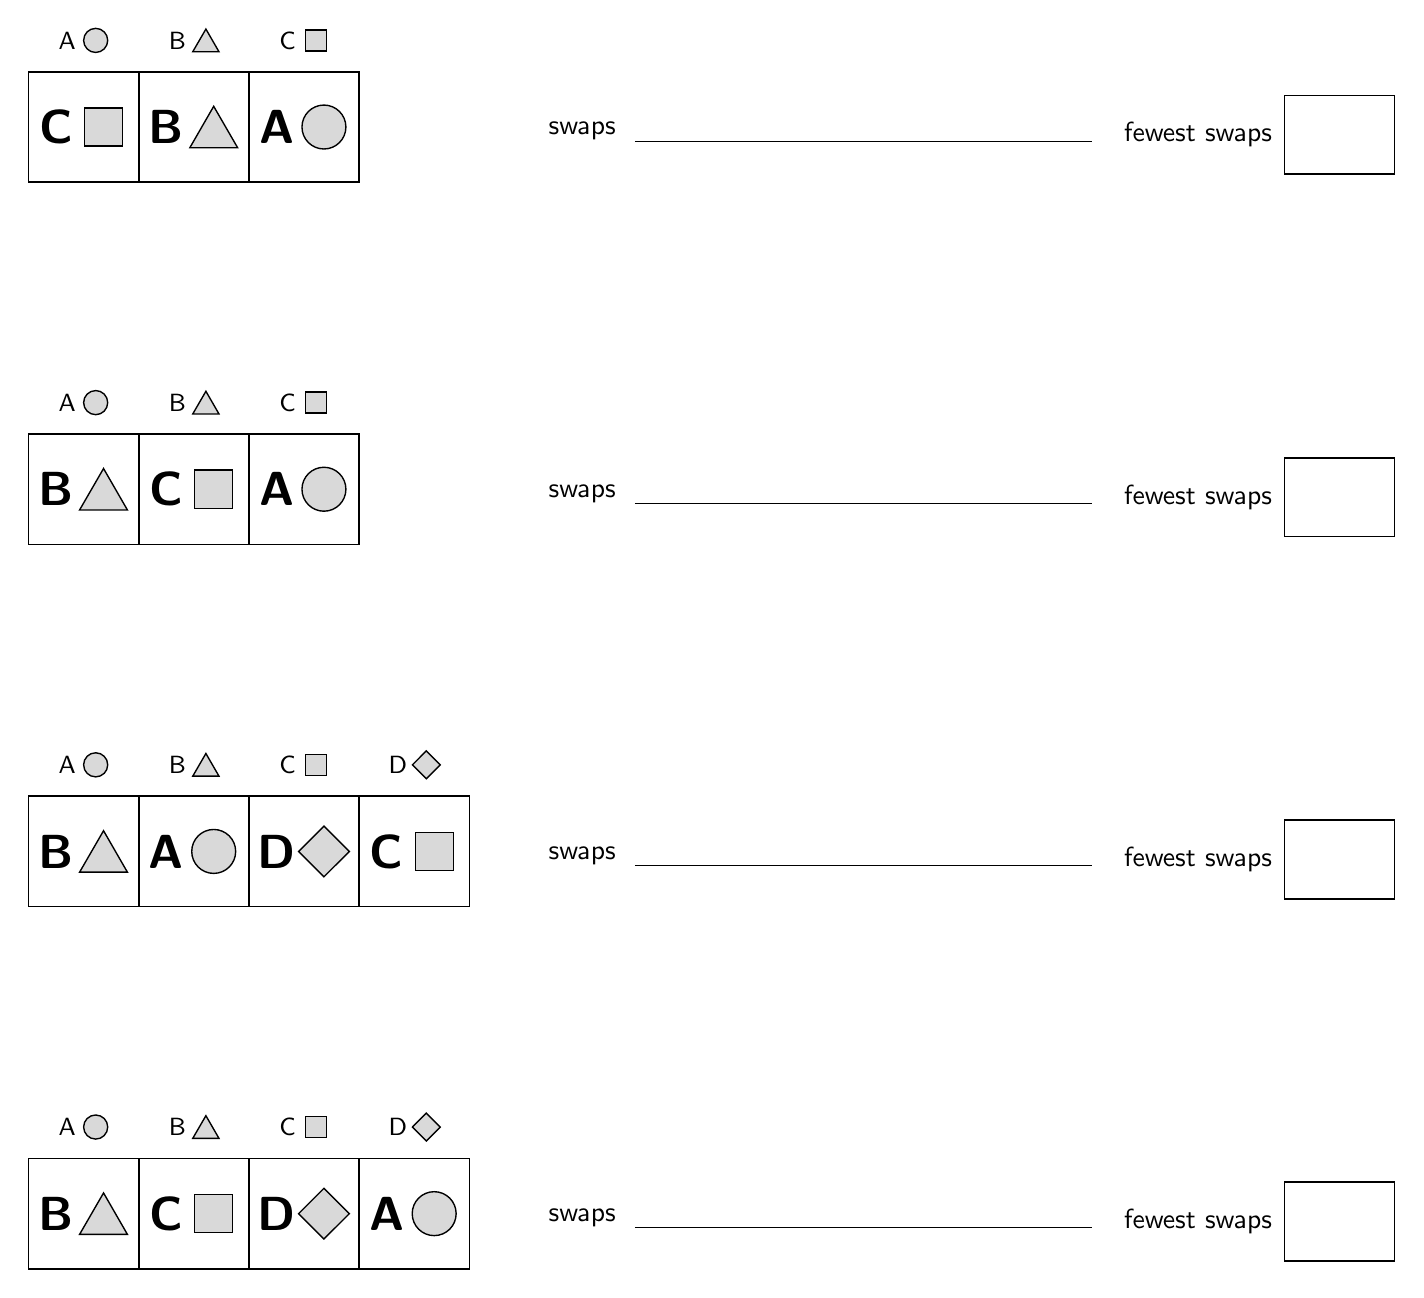
\begin{tikzpicture}[x=1mm, y=1mm]
\draw[line width=0.6pt] (0,0) rectangle (14,14);
\node[inner sep=0, font=\fontsize{9}{10.8}\selectfont] at (4.9,18) {A};
\path[fill=gray!30, draw=black, line width=0.5pt] (8.53,18) circle (1.53);
\node[inner sep=0, font=\fontsize{17}{20.4}\selectfont\bfseries] at (3.5,7) {C};
\path[fill=gray!30, draw=black, line width=0.5pt] (7.11,4.58) rectangle (11.94,9.42);
\draw[line width=0.6pt] (14,0) rectangle (28,14);
\node[inner sep=0, font=\fontsize{9}{10.8}\selectfont] at (18.9,18) {B};
\path[fill=gray!30, draw=black, line width=0.5pt] (22.53,19.44) -- (20.86,16.56) -- (24.19,16.56) -- cycle;
\node[inner sep=0, font=\fontsize{17}{20.4}\selectfont\bfseries] at (17.5,7) {B};
\path[fill=gray!30, draw=black, line width=0.5pt] (23.52,9.63) -- (20.49,4.37) -- (26.56,4.37) -- cycle;
\draw[line width=0.6pt] (28,0) rectangle (42,14);
\node[inner sep=0, font=\fontsize{9}{10.8}\selectfont] at (32.9,18) {C};
\path[fill=gray!30, draw=black, line width=0.5pt] (35.2,16.67) rectangle (37.85,19.33);
\node[inner sep=0, font=\fontsize{17}{20.4}\selectfont\bfseries] at (31.5,7) {A};
\path[fill=gray!30, draw=black, line width=0.5pt] (37.52,7) circle (2.79);
\node[anchor=base west, inner sep=0, font=\fontsize{10}{12.0}\selectfont] at (66,6) {swaps};
\draw[line width=0.4pt] (77,5.2) -- (135,5.2);
\node[anchor=east, inner sep=0, font=\fontsize{10}{12.0}\selectfont] at (158,6) {fewest swaps};
\draw[line width=0.6pt] (159.5,1) rectangle (173.5,11);
\draw[line width=0.6pt] (0,-46) rectangle (14,-32);
\node[inner sep=0, font=\fontsize{9}{10.8}\selectfont] at (4.9,-28) {A};
\path[fill=gray!30, draw=black, line width=0.5pt] (8.53,-28) circle (1.53);
\node[inner sep=0, font=\fontsize{17}{20.4}\selectfont\bfseries] at (3.5,-39) {B};
\path[fill=gray!30, draw=black, line width=0.5pt] (9.53,-36.37) -- (6.49,-41.63) -- (12.56,-41.63) -- cycle;
\draw[line width=0.6pt] (14,-46) rectangle (28,-32);
\node[inner sep=0, font=\fontsize{9}{10.8}\selectfont] at (18.9,-28) {B};
\path[fill=gray!30, draw=black, line width=0.5pt] (22.53,-26.56) -- (20.86,-29.44) -- (24.19,-29.44) -- cycle;
\node[inner sep=0, font=\fontsize{17}{20.4}\selectfont\bfseries] at (17.5,-39) {C};
\path[fill=gray!30, draw=black, line width=0.5pt] (21.11,-41.42) rectangle (25.94,-36.58);
\draw[line width=0.6pt] (28,-46) rectangle (42,-32);
\node[inner sep=0, font=\fontsize{9}{10.8}\selectfont] at (32.9,-28) {C};
\path[fill=gray!30, draw=black, line width=0.5pt] (35.2,-29.33) rectangle (37.85,-26.67);
\node[inner sep=0, font=\fontsize{17}{20.4}\selectfont\bfseries] at (31.5,-39) {A};
\path[fill=gray!30, draw=black, line width=0.5pt] (37.52,-39) circle (2.79);
\node[anchor=base west, inner sep=0, font=\fontsize{10}{12.0}\selectfont] at (66,-40) {swaps};
\draw[line width=0.4pt] (77,-40.8) -- (135,-40.8);
\node[anchor=east, inner sep=0, font=\fontsize{10}{12.0}\selectfont] at (158,-40) {fewest swaps};
\draw[line width=0.6pt] (159.5,-45) rectangle (173.5,-35);
\draw[line width=0.6pt] (0,-92) rectangle (14,-78);
\node[inner sep=0, font=\fontsize{9}{10.8}\selectfont] at (4.9,-74) {A};
\path[fill=gray!30, draw=black, line width=0.5pt] (8.53,-74) circle (1.53);
\node[inner sep=0, font=\fontsize{17}{20.4}\selectfont\bfseries] at (3.5,-85) {B};
\path[fill=gray!30, draw=black, line width=0.5pt] (9.53,-82.37) -- (6.49,-87.63) -- (12.56,-87.63) -- cycle;
\draw[line width=0.6pt] (14,-92) rectangle (28,-78);
\node[inner sep=0, font=\fontsize{9}{10.8}\selectfont] at (18.9,-74) {B};
\path[fill=gray!30, draw=black, line width=0.5pt] (22.53,-72.56) -- (20.86,-75.44) -- (24.19,-75.44) -- cycle;
\node[inner sep=0, font=\fontsize{17}{20.4}\selectfont\bfseries] at (17.5,-85) {A};
\path[fill=gray!30, draw=black, line width=0.5pt] (23.52,-85) circle (2.79);
\draw[line width=0.6pt] (28,-92) rectangle (42,-78);
\node[inner sep=0, font=\fontsize{9}{10.8}\selectfont] at (32.9,-74) {C};
\path[fill=gray!30, draw=black, line width=0.5pt] (35.2,-75.33) rectangle (37.85,-72.67);
\node[inner sep=0, font=\fontsize{17}{20.4}\selectfont\bfseries] at (31.5,-85) {D};
\path[fill=gray!30, draw=black, line width=0.5pt] (37.52,-81.78) -- (40.75,-85) -- (37.52,-88.22) -- (34.3,-85) -- cycle;
\draw[line width=0.6pt] (42,-92) rectangle (56,-78);
\node[inner sep=0, font=\fontsize{9}{10.8}\selectfont] at (46.9,-74) {D};
\path[fill=gray!30, draw=black, line width=0.5pt] (50.52,-72.23) -- (52.29,-74) -- (50.52,-75.77) -- (48.76,-74) -- cycle;
\node[inner sep=0, font=\fontsize{17}{20.4}\selectfont\bfseries] at (45.5,-85) {C};
\path[fill=gray!30, draw=black, line width=0.5pt] (49.11,-87.42) rectangle (53.94,-82.58);
\node[anchor=base west, inner sep=0, font=\fontsize{10}{12.0}\selectfont] at (66,-86) {swaps};
\draw[line width=0.4pt] (77,-86.8) -- (135,-86.8);
\node[anchor=east, inner sep=0, font=\fontsize{10}{12.0}\selectfont] at (158,-86) {fewest swaps};
\draw[line width=0.6pt] (159.5,-91) rectangle (173.5,-81);
\draw[line width=0.6pt] (0,-138) rectangle (14,-124);
\node[inner sep=0, font=\fontsize{9}{10.8}\selectfont] at (4.9,-120) {A};
\path[fill=gray!30, draw=black, line width=0.5pt] (8.53,-120) circle (1.53);
\node[inner sep=0, font=\fontsize{17}{20.4}\selectfont\bfseries] at (3.5,-131) {B};
\path[fill=gray!30, draw=black, line width=0.5pt] (9.53,-128.37) -- (6.49,-133.63) -- (12.56,-133.63) -- cycle;
\draw[line width=0.6pt] (14,-138) rectangle (28,-124);
\node[inner sep=0, font=\fontsize{9}{10.8}\selectfont] at (18.9,-120) {B};
\path[fill=gray!30, draw=black, line width=0.5pt] (22.53,-118.56) -- (20.86,-121.44) -- (24.19,-121.44) -- cycle;
\node[inner sep=0, font=\fontsize{17}{20.4}\selectfont\bfseries] at (17.5,-131) {C};
\path[fill=gray!30, draw=black, line width=0.5pt] (21.11,-133.42) rectangle (25.94,-128.58);
\draw[line width=0.6pt] (28,-138) rectangle (42,-124);
\node[inner sep=0, font=\fontsize{9}{10.8}\selectfont] at (32.9,-120) {C};
\path[fill=gray!30, draw=black, line width=0.5pt] (35.2,-121.33) rectangle (37.85,-118.67);
\node[inner sep=0, font=\fontsize{17}{20.4}\selectfont\bfseries] at (31.5,-131) {D};
\path[fill=gray!30, draw=black, line width=0.5pt] (37.52,-127.78) -- (40.75,-131) -- (37.52,-134.22) -- (34.3,-131) -- cycle;
\draw[line width=0.6pt] (42,-138) rectangle (56,-124);
\node[inner sep=0, font=\fontsize{9}{10.8}\selectfont] at (46.9,-120) {D};
\path[fill=gray!30, draw=black, line width=0.5pt] (50.52,-118.23) -- (52.29,-120) -- (50.52,-121.77) -- (48.76,-120) -- cycle;
\node[inner sep=0, font=\fontsize{17}{20.4}\selectfont\bfseries] at (45.5,-131) {A};
\path[fill=gray!30, draw=black, line width=0.5pt] (51.52,-131) circle (2.79);
\node[anchor=base west, inner sep=0, font=\fontsize{10}{12.0}\selectfont] at (66,-132) {swaps};
\draw[line width=0.4pt] (77,-132.8) -- (135,-132.8);
\node[anchor=east, inner sep=0, font=\fontsize{10}{12.0}\selectfont] at (158,-132) {fewest swaps};
\draw[line width=0.6pt] (159.5,-137) rectangle (173.5,-127);
\end{tikzpicture}\par

\vfill
\newpage
\prob{5} Put a counter on every letter at home on the six A--C outcome cards. Are there more counters, more outcome cards, or the same number, and how many counters does each letter get?

\par\vspace{3mm}\noindent\hspace*{6mm}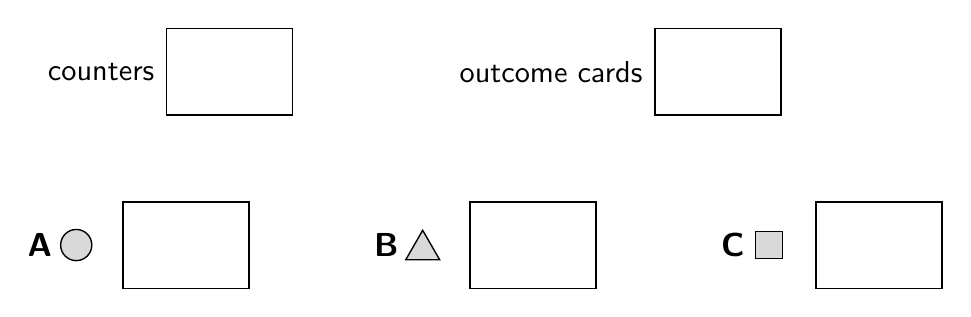
\begin{tikzpicture}[x=1mm, y=1mm]
\node[anchor=east, inner sep=0, font=\fontsize{11}{13.2}\selectfont] at (22,5.5) {counters};
\draw[line width=0.6pt] (23.5,0) rectangle (39.5,11);
\node[anchor=east, inner sep=0, font=\fontsize{11}{13.2}\selectfont] at (84,5.5) {outcome cards};
\draw[line width=0.6pt] (85.5,0) rectangle (101.5,11);
\node[inner sep=0, font=\fontsize{13}{15.6}\selectfont\bfseries] at (7.4,-16.5) {A};
\path[fill=gray!30, draw=black, line width=0.5pt] (12.02,-16.5) circle (1.98);
\draw[line width=0.6pt] (18,-22) rectangle (34,-11);
\node[inner sep=0, font=\fontsize{13}{15.6}\selectfont\bfseries] at (51.4,-16.5) {B};
\path[fill=gray!30, draw=black, line width=0.5pt] (56.02,-14.63) -- (53.87,-18.37) -- (58.18,-18.37) -- cycle;
\draw[line width=0.6pt] (62,-22) rectangle (78,-11);
\node[inner sep=0, font=\fontsize{13}{15.6}\selectfont\bfseries] at (95.4,-16.5) {C};
\path[fill=gray!30, draw=black, line width=0.5pt] (98.31,-18.22) rectangle (101.74,-14.78);
\draw[line width=0.6pt] (106,-22) rectangle (122,-11);
\end{tikzpicture}\par

\vspace{26mm}
\prob{6} A card may not go in a home that shows its picture crossed out. Find every way to put A, B and C in these homes.

\par\vspace{3mm}\noindent\hspace*{2mm}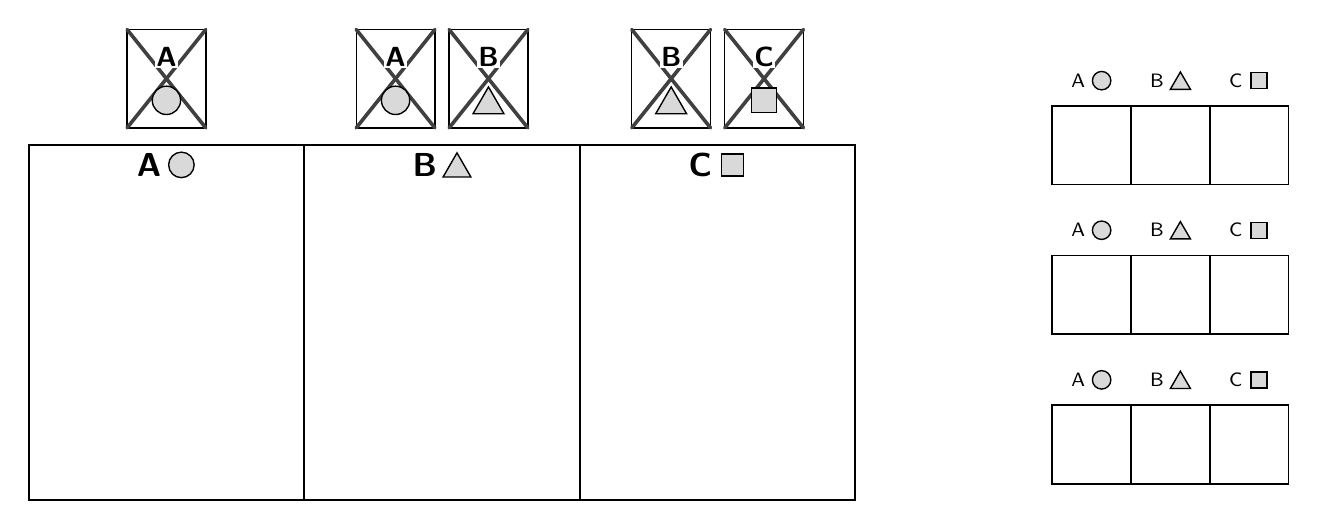
\begin{tikzpicture}[x=1mm, y=1mm]
\draw[line width=0.7pt] (0,0) rectangle (35,45);
\node[inner sep=0, font=\fontsize{12}{14.4}\selectfont\bfseries] at (15.3,42.5) {A};
\path[fill=gray!30, draw=black, line width=0.5pt] (19.4,42.5) circle (1.62);
\draw[line width=0.5pt, draw=black, fill=white] (12.5,47.2) rectangle (22.5,59.7);
\draw[line width=1.3pt, draw=black!75, line cap=round] (12.5,47.2) -- (22.5,59.7);
\draw[line width=1.3pt, draw=black!75, line cap=round] (12.5,59.7) -- (22.5,47.2);
\node[inner sep=0.5pt, fill=white, text=black, font=\fontsize{10}{12.0}\selectfont\bfseries] at (17.5,56.2) {A};
\path[fill=gray!30, draw=black, line width=0.5pt] (17.5,50.7) circle (1.8);
\draw[line width=0.7pt] (35,0) rectangle (70,45);
\node[inner sep=0, font=\fontsize{12}{14.4}\selectfont\bfseries] at (50.3,42.5) {B};
\path[fill=gray!30, draw=black, line width=0.5pt] (54.4,44.03) -- (52.64,40.97) -- (56.16,40.97) -- cycle;
\draw[line width=0.5pt, draw=black, fill=white] (41.6,47.2) rectangle (51.6,59.7);
\draw[line width=1.3pt, draw=black!75, line cap=round] (41.6,47.2) -- (51.6,59.7);
\draw[line width=1.3pt, draw=black!75, line cap=round] (41.6,59.7) -- (51.6,47.2);
\node[inner sep=0.5pt, fill=white, text=black, font=\fontsize{10}{12.0}\selectfont\bfseries] at (46.6,56.2) {A};
\path[fill=gray!30, draw=black, line width=0.5pt] (46.6,50.7) circle (1.8);
\draw[line width=0.5pt, draw=black, fill=white] (53.4,47.2) rectangle (63.4,59.7);
\draw[line width=1.3pt, draw=black!75, line cap=round] (53.4,47.2) -- (63.4,59.7);
\draw[line width=1.3pt, draw=black!75, line cap=round] (53.4,59.7) -- (63.4,47.2);
\node[inner sep=0.5pt, fill=white, text=black, font=\fontsize{10}{12.0}\selectfont\bfseries] at (58.4,56.2) {B};
\path[fill=gray!30, draw=black, line width=0.5pt] (58.4,52.4) -- (56.44,49) -- (60.36,49) -- cycle;
\draw[line width=0.7pt] (70,0) rectangle (105,45);
\node[inner sep=0, font=\fontsize{12}{14.4}\selectfont\bfseries] at (85.3,42.5) {C};
\path[fill=gray!30, draw=black, line width=0.5pt] (88,41.1) rectangle (90.8,43.9);
\draw[line width=0.5pt, draw=black, fill=white] (76.6,47.2) rectangle (86.6,59.7);
\draw[line width=1.3pt, draw=black!75, line cap=round] (76.6,47.2) -- (86.6,59.7);
\draw[line width=1.3pt, draw=black!75, line cap=round] (76.6,59.7) -- (86.6,47.2);
\node[inner sep=0.5pt, fill=white, text=black, font=\fontsize{10}{12.0}\selectfont\bfseries] at (81.6,56.2) {B};
\path[fill=gray!30, draw=black, line width=0.5pt] (81.6,52.4) -- (79.64,49) -- (83.56,49) -- cycle;
\draw[line width=0.5pt, draw=black, fill=white] (88.4,47.2) rectangle (98.4,59.7);
\draw[line width=1.3pt, draw=black!75, line cap=round] (88.4,47.2) -- (98.4,59.7);
\draw[line width=1.3pt, draw=black!75, line cap=round] (88.4,59.7) -- (98.4,47.2);
\node[inner sep=0.5pt, fill=white, text=black, font=\fontsize{10}{12.0}\selectfont\bfseries] at (93.4,56.2) {C};
\path[fill=gray!30, draw=black, line width=0.5pt] (91.84,49.14) rectangle (94.96,52.26);
\draw[line width=0.6pt] (130,40) rectangle (140,50);
\node[inner sep=0, font=\fontsize{7}{8.4}\selectfont] at (133.3,53.2) {A};
\path[fill=gray!30, draw=black, line width=0.5pt] (136.27,53.2) circle (1.17);
\draw[line width=0.6pt] (140,40) rectangle (150,50);
\node[inner sep=0, font=\fontsize{7}{8.4}\selectfont] at (143.3,53.2) {B};
\path[fill=gray!30, draw=black, line width=0.5pt] (146.27,54.3) -- (145,52.1) -- (147.55,52.1) -- cycle;
\draw[line width=0.6pt] (150,40) rectangle (160,50);
\node[inner sep=0, font=\fontsize{7}{8.4}\selectfont] at (153.3,53.2) {C};
\path[fill=gray!30, draw=black, line width=0.5pt] (155.26,52.19) rectangle (157.29,54.21);
\draw[line width=0.6pt] (130,21) rectangle (140,31);
\node[inner sep=0, font=\fontsize{7}{8.4}\selectfont] at (133.3,34.2) {A};
\path[fill=gray!30, draw=black, line width=0.5pt] (136.27,34.2) circle (1.17);
\draw[line width=0.6pt] (140,21) rectangle (150,31);
\node[inner sep=0, font=\fontsize{7}{8.4}\selectfont] at (143.3,34.2) {B};
\path[fill=gray!30, draw=black, line width=0.5pt] (146.27,35.3) -- (145,33.1) -- (147.55,33.1) -- cycle;
\draw[line width=0.6pt] (150,21) rectangle (160,31);
\node[inner sep=0, font=\fontsize{7}{8.4}\selectfont] at (153.3,34.2) {C};
\path[fill=gray!30, draw=black, line width=0.5pt] (155.26,33.19) rectangle (157.29,35.21);
\draw[line width=0.6pt] (130,2) rectangle (140,12);
\node[inner sep=0, font=\fontsize{7}{8.4}\selectfont] at (133.3,15.2) {A};
\path[fill=gray!30, draw=black, line width=0.5pt] (136.27,15.2) circle (1.17);
\draw[line width=0.6pt] (140,2) rectangle (150,12);
\node[inner sep=0, font=\fontsize{7}{8.4}\selectfont] at (143.3,15.2) {B};
\path[fill=gray!30, draw=black, line width=0.5pt] (146.27,16.3) -- (145,14.1) -- (147.55,14.1) -- cycle;
\draw[line width=0.6pt] (150,2) rectangle (160,12);
\node[inner sep=0, font=\fontsize{7}{8.4}\selectfont] at (153.3,15.2) {C};
\path[fill=gray!30, draw=black, line width=0.5pt] (155.26,14.19) rectangle (157.29,16.21);
\end{tikzpicture}\par

\vfill
\newpage
\prob{7} Find every way to put A, B, C and D in these homes.

\par\vspace{3mm}\noindent\hspace*{2mm}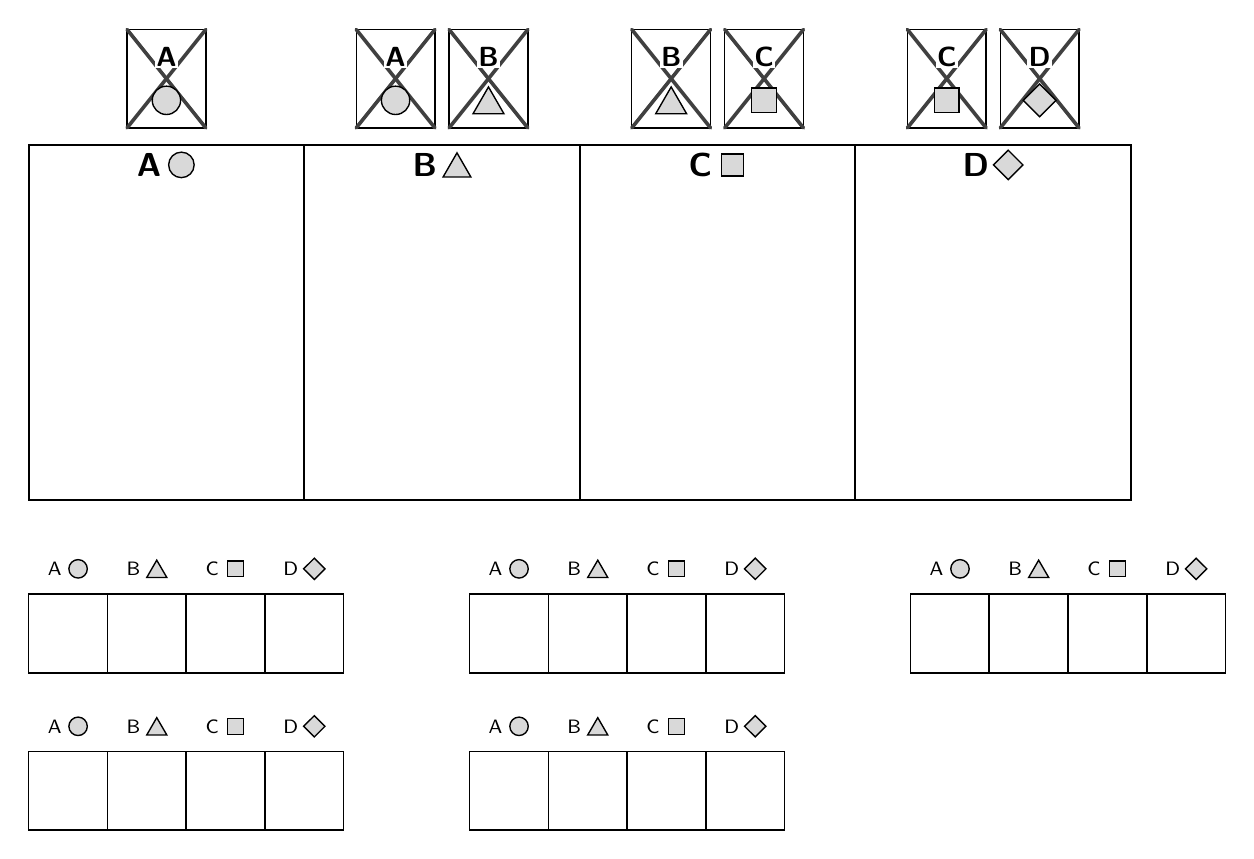
\begin{tikzpicture}[x=1mm, y=1mm]
\draw[line width=0.7pt] (0,0) rectangle (35,45);
\node[inner sep=0, font=\fontsize{12}{14.4}\selectfont\bfseries] at (15.3,42.5) {A};
\path[fill=gray!30, draw=black, line width=0.5pt] (19.4,42.5) circle (1.62);
\draw[line width=0.5pt, draw=black, fill=white] (12.5,47.2) rectangle (22.5,59.7);
\draw[line width=1.3pt, draw=black!75, line cap=round] (12.5,47.2) -- (22.5,59.7);
\draw[line width=1.3pt, draw=black!75, line cap=round] (12.5,59.7) -- (22.5,47.2);
\node[inner sep=0.5pt, fill=white, text=black, font=\fontsize{10}{12.0}\selectfont\bfseries] at (17.5,56.2) {A};
\path[fill=gray!30, draw=black, line width=0.5pt] (17.5,50.7) circle (1.8);
\draw[line width=0.7pt] (35,0) rectangle (70,45);
\node[inner sep=0, font=\fontsize{12}{14.4}\selectfont\bfseries] at (50.3,42.5) {B};
\path[fill=gray!30, draw=black, line width=0.5pt] (54.4,44.03) -- (52.64,40.97) -- (56.16,40.97) -- cycle;
\draw[line width=0.5pt, draw=black, fill=white] (41.6,47.2) rectangle (51.6,59.7);
\draw[line width=1.3pt, draw=black!75, line cap=round] (41.6,47.2) -- (51.6,59.7);
\draw[line width=1.3pt, draw=black!75, line cap=round] (41.6,59.7) -- (51.6,47.2);
\node[inner sep=0.5pt, fill=white, text=black, font=\fontsize{10}{12.0}\selectfont\bfseries] at (46.6,56.2) {A};
\path[fill=gray!30, draw=black, line width=0.5pt] (46.6,50.7) circle (1.8);
\draw[line width=0.5pt, draw=black, fill=white] (53.4,47.2) rectangle (63.4,59.7);
\draw[line width=1.3pt, draw=black!75, line cap=round] (53.4,47.2) -- (63.4,59.7);
\draw[line width=1.3pt, draw=black!75, line cap=round] (53.4,59.7) -- (63.4,47.2);
\node[inner sep=0.5pt, fill=white, text=black, font=\fontsize{10}{12.0}\selectfont\bfseries] at (58.4,56.2) {B};
\path[fill=gray!30, draw=black, line width=0.5pt] (58.4,52.4) -- (56.44,49) -- (60.36,49) -- cycle;
\draw[line width=0.7pt] (70,0) rectangle (105,45);
\node[inner sep=0, font=\fontsize{12}{14.4}\selectfont\bfseries] at (85.3,42.5) {C};
\path[fill=gray!30, draw=black, line width=0.5pt] (88,41.1) rectangle (90.8,43.9);
\draw[line width=0.5pt, draw=black, fill=white] (76.6,47.2) rectangle (86.6,59.7);
\draw[line width=1.3pt, draw=black!75, line cap=round] (76.6,47.2) -- (86.6,59.7);
\draw[line width=1.3pt, draw=black!75, line cap=round] (76.6,59.7) -- (86.6,47.2);
\node[inner sep=0.5pt, fill=white, text=black, font=\fontsize{10}{12.0}\selectfont\bfseries] at (81.6,56.2) {B};
\path[fill=gray!30, draw=black, line width=0.5pt] (81.6,52.4) -- (79.64,49) -- (83.56,49) -- cycle;
\draw[line width=0.5pt, draw=black, fill=white] (88.4,47.2) rectangle (98.4,59.7);
\draw[line width=1.3pt, draw=black!75, line cap=round] (88.4,47.2) -- (98.4,59.7);
\draw[line width=1.3pt, draw=black!75, line cap=round] (88.4,59.7) -- (98.4,47.2);
\node[inner sep=0.5pt, fill=white, text=black, font=\fontsize{10}{12.0}\selectfont\bfseries] at (93.4,56.2) {C};
\path[fill=gray!30, draw=black, line width=0.5pt] (91.84,49.14) rectangle (94.96,52.26);
\draw[line width=0.7pt] (105,0) rectangle (140,45);
\node[inner sep=0, font=\fontsize{12}{14.4}\selectfont\bfseries] at (120.3,42.5) {D};
\path[fill=gray!30, draw=black, line width=0.5pt] (124.4,44.37) -- (126.27,42.5) -- (124.4,40.63) -- (122.53,42.5) -- cycle;
\draw[line width=0.5pt, draw=black, fill=white] (111.6,47.2) rectangle (121.6,59.7);
\draw[line width=1.3pt, draw=black!75, line cap=round] (111.6,47.2) -- (121.6,59.7);
\draw[line width=1.3pt, draw=black!75, line cap=round] (111.6,59.7) -- (121.6,47.2);
\node[inner sep=0.5pt, fill=white, text=black, font=\fontsize{10}{12.0}\selectfont\bfseries] at (116.6,56.2) {C};
\path[fill=gray!30, draw=black, line width=0.5pt] (115.04,49.14) rectangle (118.16,52.26);
\draw[line width=0.5pt, draw=black, fill=white] (123.4,47.2) rectangle (133.4,59.7);
\draw[line width=1.3pt, draw=black!75, line cap=round] (123.4,47.2) -- (133.4,59.7);
\draw[line width=1.3pt, draw=black!75, line cap=round] (123.4,59.7) -- (133.4,47.2);
\node[inner sep=0.5pt, fill=white, text=black, font=\fontsize{10}{12.0}\selectfont\bfseries] at (128.4,56.2) {D};
\path[fill=gray!30, draw=black, line width=0.5pt] (128.4,52.78) -- (130.48,50.7) -- (128.4,48.62) -- (126.32,50.7) -- cycle;
\draw[line width=0.6pt] (0,-22) rectangle (10,-12);
\node[inner sep=0, font=\fontsize{7}{8.4}\selectfont] at (3.3,-8.8) {A};
\path[fill=gray!30, draw=black, line width=0.5pt] (6.28,-8.8) circle (1.17);
\draw[line width=0.6pt] (10,-22) rectangle (20,-12);
\node[inner sep=0, font=\fontsize{7}{8.4}\selectfont] at (13.3,-8.8) {B};
\path[fill=gray!30, draw=black, line width=0.5pt] (16.27,-7.7) -- (15,-9.9) -- (17.55,-9.9) -- cycle;
\draw[line width=0.6pt] (20,-22) rectangle (30,-12);
\node[inner sep=0, font=\fontsize{7}{8.4}\selectfont] at (23.3,-8.8) {C};
\path[fill=gray!30, draw=black, line width=0.5pt] (25.26,-9.81) rectangle (27.29,-7.79);
\draw[line width=0.6pt] (30,-22) rectangle (40,-12);
\node[inner sep=0, font=\fontsize{7}{8.4}\selectfont] at (33.3,-8.8) {D};
\path[fill=gray!30, draw=black, line width=0.5pt] (36.28,-7.45) -- (37.63,-8.8) -- (36.28,-10.15) -- (34.92,-8.8) -- cycle;
\draw[line width=0.6pt] (56,-22) rectangle (66,-12);
\node[inner sep=0, font=\fontsize{7}{8.4}\selectfont] at (59.3,-8.8) {A};
\path[fill=gray!30, draw=black, line width=0.5pt] (62.28,-8.8) circle (1.17);
\draw[line width=0.6pt] (66,-22) rectangle (76,-12);
\node[inner sep=0, font=\fontsize{7}{8.4}\selectfont] at (69.3,-8.8) {B};
\path[fill=gray!30, draw=black, line width=0.5pt] (72.28,-7.7) -- (71,-9.9) -- (73.55,-9.9) -- cycle;
\draw[line width=0.6pt] (76,-22) rectangle (86,-12);
\node[inner sep=0, font=\fontsize{7}{8.4}\selectfont] at (79.3,-8.8) {C};
\path[fill=gray!30, draw=black, line width=0.5pt] (81.26,-9.81) rectangle (83.29,-7.79);
\draw[line width=0.6pt] (86,-22) rectangle (96,-12);
\node[inner sep=0, font=\fontsize{7}{8.4}\selectfont] at (89.3,-8.8) {D};
\path[fill=gray!30, draw=black, line width=0.5pt] (92.28,-7.45) -- (93.63,-8.8) -- (92.28,-10.15) -- (90.92,-8.8) -- cycle;
\draw[line width=0.6pt] (112,-22) rectangle (122,-12);
\node[inner sep=0, font=\fontsize{7}{8.4}\selectfont] at (115.3,-8.8) {A};
\path[fill=gray!30, draw=black, line width=0.5pt] (118.28,-8.8) circle (1.17);
\draw[line width=0.6pt] (122,-22) rectangle (132,-12);
\node[inner sep=0, font=\fontsize{7}{8.4}\selectfont] at (125.3,-8.8) {B};
\path[fill=gray!30, draw=black, line width=0.5pt] (128.27,-7.7) -- (127,-9.9) -- (129.55,-9.9) -- cycle;
\draw[line width=0.6pt] (132,-22) rectangle (142,-12);
\node[inner sep=0, font=\fontsize{7}{8.4}\selectfont] at (135.3,-8.8) {C};
\path[fill=gray!30, draw=black, line width=0.5pt] (137.26,-9.81) rectangle (139.29,-7.79);
\draw[line width=0.6pt] (142,-22) rectangle (152,-12);
\node[inner sep=0, font=\fontsize{7}{8.4}\selectfont] at (145.3,-8.8) {D};
\path[fill=gray!30, draw=black, line width=0.5pt] (148.27,-7.45) -- (149.63,-8.8) -- (148.27,-10.15) -- (146.92,-8.8) -- cycle;
\draw[line width=0.6pt] (0,-42) rectangle (10,-32);
\node[inner sep=0, font=\fontsize{7}{8.4}\selectfont] at (3.3,-28.8) {A};
\path[fill=gray!30, draw=black, line width=0.5pt] (6.28,-28.8) circle (1.17);
\draw[line width=0.6pt] (10,-42) rectangle (20,-32);
\node[inner sep=0, font=\fontsize{7}{8.4}\selectfont] at (13.3,-28.8) {B};
\path[fill=gray!30, draw=black, line width=0.5pt] (16.27,-27.7) -- (15,-29.9) -- (17.55,-29.9) -- cycle;
\draw[line width=0.6pt] (20,-42) rectangle (30,-32);
\node[inner sep=0, font=\fontsize{7}{8.4}\selectfont] at (23.3,-28.8) {C};
\path[fill=gray!30, draw=black, line width=0.5pt] (25.26,-29.81) rectangle (27.29,-27.79);
\draw[line width=0.6pt] (30,-42) rectangle (40,-32);
\node[inner sep=0, font=\fontsize{7}{8.4}\selectfont] at (33.3,-28.8) {D};
\path[fill=gray!30, draw=black, line width=0.5pt] (36.28,-27.45) -- (37.63,-28.8) -- (36.28,-30.15) -- (34.92,-28.8) -- cycle;
\draw[line width=0.6pt] (56,-42) rectangle (66,-32);
\node[inner sep=0, font=\fontsize{7}{8.4}\selectfont] at (59.3,-28.8) {A};
\path[fill=gray!30, draw=black, line width=0.5pt] (62.28,-28.8) circle (1.17);
\draw[line width=0.6pt] (66,-42) rectangle (76,-32);
\node[inner sep=0, font=\fontsize{7}{8.4}\selectfont] at (69.3,-28.8) {B};
\path[fill=gray!30, draw=black, line width=0.5pt] (72.28,-27.7) -- (71,-29.9) -- (73.55,-29.9) -- cycle;
\draw[line width=0.6pt] (76,-42) rectangle (86,-32);
\node[inner sep=0, font=\fontsize{7}{8.4}\selectfont] at (79.3,-28.8) {C};
\path[fill=gray!30, draw=black, line width=0.5pt] (81.26,-29.81) rectangle (83.29,-27.79);
\draw[line width=0.6pt] (86,-42) rectangle (96,-32);
\node[inner sep=0, font=\fontsize{7}{8.4}\selectfont] at (89.3,-28.8) {D};
\path[fill=gray!30, draw=black, line width=0.5pt] (92.28,-27.45) -- (93.63,-28.8) -- (92.28,-30.15) -- (90.92,-28.8) -- cycle;
\end{tikzpicture}\par

\vfill
\prob{8} Find every way to put A, B, C and D in these homes.

\par\vspace{3mm}\noindent\hspace*{2mm}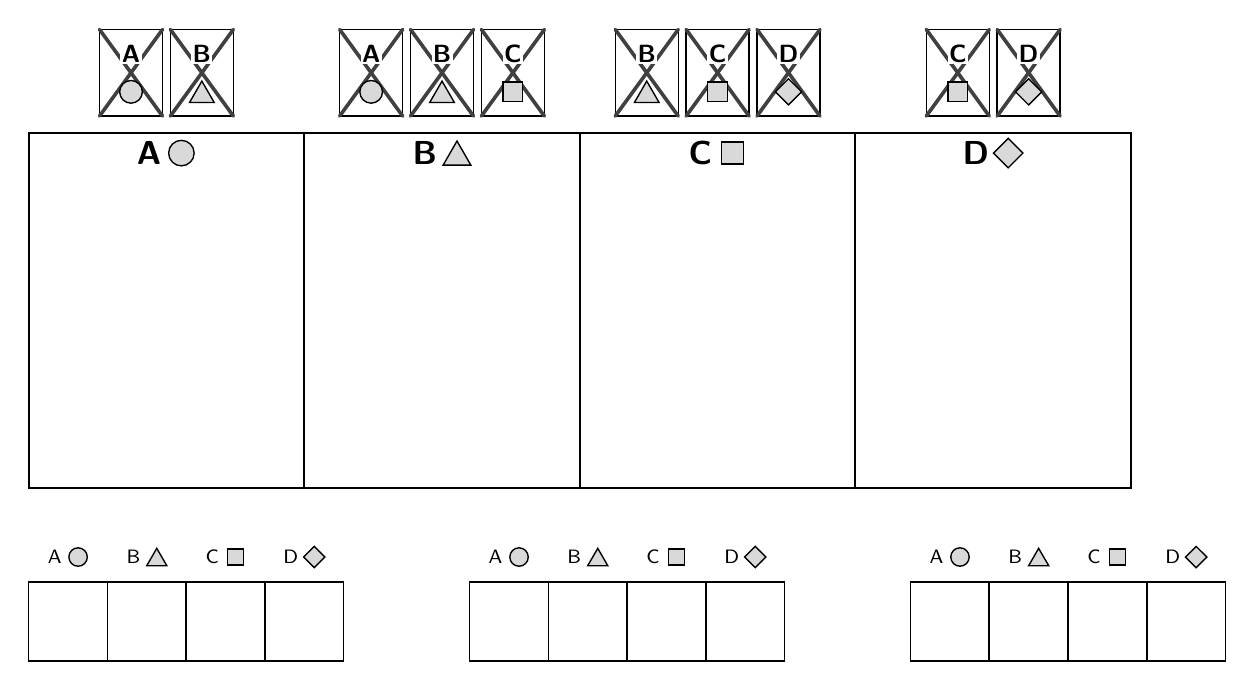
\begin{tikzpicture}[x=1mm, y=1mm]
\draw[line width=0.7pt] (0,0) rectangle (35,45);
\node[inner sep=0, font=\fontsize{12}{14.4}\selectfont\bfseries] at (15.3,42.5) {A};
\path[fill=gray!30, draw=black, line width=0.5pt] (19.4,42.5) circle (1.62);
\draw[line width=0.5pt, draw=black, fill=white] (9,47.2) rectangle (17,58.2);
\draw[line width=1.3pt, draw=black!75, line cap=round] (9,47.2) -- (17,58.2);
\draw[line width=1.3pt, draw=black!75, line cap=round] (9,58.2) -- (17,47.2);
\node[inner sep=0.5pt, fill=white, text=black, font=\fontsize{9}{10.8}\selectfont\bfseries] at (13,55.12) {A};
\path[fill=gray!30, draw=black, line width=0.5pt] (13,50.28) circle (1.44);
\draw[line width=0.5pt, draw=black, fill=white] (18,47.2) rectangle (26,58.2);
\draw[line width=1.3pt, draw=black!75, line cap=round] (18,47.2) -- (26,58.2);
\draw[line width=1.3pt, draw=black!75, line cap=round] (18,58.2) -- (26,47.2);
\node[inner sep=0.5pt, fill=white, text=black, font=\fontsize{9}{10.8}\selectfont\bfseries] at (22,55.12) {B};
\path[fill=gray!30, draw=black, line width=0.5pt] (22,51.64) -- (20.43,48.92) -- (23.57,48.92) -- cycle;
\draw[line width=0.7pt] (35,0) rectangle (70,45);
\node[inner sep=0, font=\fontsize{12}{14.4}\selectfont\bfseries] at (50.3,42.5) {B};
\path[fill=gray!30, draw=black, line width=0.5pt] (54.4,44.03) -- (52.64,40.97) -- (56.16,40.97) -- cycle;
\draw[line width=0.5pt, draw=black, fill=white] (39.5,47.2) rectangle (47.5,58.2);
\draw[line width=1.3pt, draw=black!75, line cap=round] (39.5,47.2) -- (47.5,58.2);
\draw[line width=1.3pt, draw=black!75, line cap=round] (39.5,58.2) -- (47.5,47.2);
\node[inner sep=0.5pt, fill=white, text=black, font=\fontsize{9}{10.8}\selectfont\bfseries] at (43.5,55.12) {A};
\path[fill=gray!30, draw=black, line width=0.5pt] (43.5,50.28) circle (1.44);
\draw[line width=0.5pt, draw=black, fill=white] (48.5,47.2) rectangle (56.5,58.2);
\draw[line width=1.3pt, draw=black!75, line cap=round] (48.5,47.2) -- (56.5,58.2);
\draw[line width=1.3pt, draw=black!75, line cap=round] (48.5,58.2) -- (56.5,47.2);
\node[inner sep=0.5pt, fill=white, text=black, font=\fontsize{9}{10.8}\selectfont\bfseries] at (52.5,55.12) {B};
\path[fill=gray!30, draw=black, line width=0.5pt] (52.5,51.64) -- (50.93,48.92) -- (54.07,48.92) -- cycle;
\draw[line width=0.5pt, draw=black, fill=white] (57.5,47.2) rectangle (65.5,58.2);
\draw[line width=1.3pt, draw=black!75, line cap=round] (57.5,47.2) -- (65.5,58.2);
\draw[line width=1.3pt, draw=black!75, line cap=round] (57.5,58.2) -- (65.5,47.2);
\node[inner sep=0.5pt, fill=white, text=black, font=\fontsize{9}{10.8}\selectfont\bfseries] at (61.5,55.12) {C};
\path[fill=gray!30, draw=black, line width=0.5pt] (60.25,49.03) rectangle (62.75,51.53);
\draw[line width=0.7pt] (70,0) rectangle (105,45);
\node[inner sep=0, font=\fontsize{12}{14.4}\selectfont\bfseries] at (85.3,42.5) {C};
\path[fill=gray!30, draw=black, line width=0.5pt] (88,41.1) rectangle (90.8,43.9);
\draw[line width=0.5pt, draw=black, fill=white] (74.5,47.2) rectangle (82.5,58.2);
\draw[line width=1.3pt, draw=black!75, line cap=round] (74.5,47.2) -- (82.5,58.2);
\draw[line width=1.3pt, draw=black!75, line cap=round] (74.5,58.2) -- (82.5,47.2);
\node[inner sep=0.5pt, fill=white, text=black, font=\fontsize{9}{10.8}\selectfont\bfseries] at (78.5,55.12) {B};
\path[fill=gray!30, draw=black, line width=0.5pt] (78.5,51.64) -- (76.93,48.92) -- (80.07,48.92) -- cycle;
\draw[line width=0.5pt, draw=black, fill=white] (83.5,47.2) rectangle (91.5,58.2);
\draw[line width=1.3pt, draw=black!75, line cap=round] (83.5,47.2) -- (91.5,58.2);
\draw[line width=1.3pt, draw=black!75, line cap=round] (83.5,58.2) -- (91.5,47.2);
\node[inner sep=0.5pt, fill=white, text=black, font=\fontsize{9}{10.8}\selectfont\bfseries] at (87.5,55.12) {C};
\path[fill=gray!30, draw=black, line width=0.5pt] (86.25,49.03) rectangle (88.75,51.53);
\draw[line width=0.5pt, draw=black, fill=white] (92.5,47.2) rectangle (100.5,58.2);
\draw[line width=1.3pt, draw=black!75, line cap=round] (92.5,47.2) -- (100.5,58.2);
\draw[line width=1.3pt, draw=black!75, line cap=round] (92.5,58.2) -- (100.5,47.2);
\node[inner sep=0.5pt, fill=white, text=black, font=\fontsize{9}{10.8}\selectfont\bfseries] at (96.5,55.12) {D};
\path[fill=gray!30, draw=black, line width=0.5pt] (96.5,51.94) -- (98.16,50.28) -- (96.5,48.62) -- (94.84,50.28) -- cycle;
\draw[line width=0.7pt] (105,0) rectangle (140,45);
\node[inner sep=0, font=\fontsize{12}{14.4}\selectfont\bfseries] at (120.3,42.5) {D};
\path[fill=gray!30, draw=black, line width=0.5pt] (124.4,44.37) -- (126.27,42.5) -- (124.4,40.63) -- (122.53,42.5) -- cycle;
\draw[line width=0.5pt, draw=black, fill=white] (114,47.2) rectangle (122,58.2);
\draw[line width=1.3pt, draw=black!75, line cap=round] (114,47.2) -- (122,58.2);
\draw[line width=1.3pt, draw=black!75, line cap=round] (114,58.2) -- (122,47.2);
\node[inner sep=0.5pt, fill=white, text=black, font=\fontsize{9}{10.8}\selectfont\bfseries] at (118,55.12) {C};
\path[fill=gray!30, draw=black, line width=0.5pt] (116.75,49.03) rectangle (119.25,51.53);
\draw[line width=0.5pt, draw=black, fill=white] (123,47.2) rectangle (131,58.2);
\draw[line width=1.3pt, draw=black!75, line cap=round] (123,47.2) -- (131,58.2);
\draw[line width=1.3pt, draw=black!75, line cap=round] (123,58.2) -- (131,47.2);
\node[inner sep=0.5pt, fill=white, text=black, font=\fontsize{9}{10.8}\selectfont\bfseries] at (127,55.12) {D};
\path[fill=gray!30, draw=black, line width=0.5pt] (127,51.94) -- (128.66,50.28) -- (127,48.62) -- (125.34,50.28) -- cycle;
\draw[line width=0.6pt] (0,-22) rectangle (10,-12);
\node[inner sep=0, font=\fontsize{7}{8.4}\selectfont] at (3.3,-8.8) {A};
\path[fill=gray!30, draw=black, line width=0.5pt] (6.28,-8.8) circle (1.17);
\draw[line width=0.6pt] (10,-22) rectangle (20,-12);
\node[inner sep=0, font=\fontsize{7}{8.4}\selectfont] at (13.3,-8.8) {B};
\path[fill=gray!30, draw=black, line width=0.5pt] (16.27,-7.7) -- (15,-9.9) -- (17.55,-9.9) -- cycle;
\draw[line width=0.6pt] (20,-22) rectangle (30,-12);
\node[inner sep=0, font=\fontsize{7}{8.4}\selectfont] at (23.3,-8.8) {C};
\path[fill=gray!30, draw=black, line width=0.5pt] (25.26,-9.81) rectangle (27.29,-7.79);
\draw[line width=0.6pt] (30,-22) rectangle (40,-12);
\node[inner sep=0, font=\fontsize{7}{8.4}\selectfont] at (33.3,-8.8) {D};
\path[fill=gray!30, draw=black, line width=0.5pt] (36.28,-7.45) -- (37.63,-8.8) -- (36.28,-10.15) -- (34.92,-8.8) -- cycle;
\draw[line width=0.6pt] (56,-22) rectangle (66,-12);
\node[inner sep=0, font=\fontsize{7}{8.4}\selectfont] at (59.3,-8.8) {A};
\path[fill=gray!30, draw=black, line width=0.5pt] (62.28,-8.8) circle (1.17);
\draw[line width=0.6pt] (66,-22) rectangle (76,-12);
\node[inner sep=0, font=\fontsize{7}{8.4}\selectfont] at (69.3,-8.8) {B};
\path[fill=gray!30, draw=black, line width=0.5pt] (72.28,-7.7) -- (71,-9.9) -- (73.55,-9.9) -- cycle;
\draw[line width=0.6pt] (76,-22) rectangle (86,-12);
\node[inner sep=0, font=\fontsize{7}{8.4}\selectfont] at (79.3,-8.8) {C};
\path[fill=gray!30, draw=black, line width=0.5pt] (81.26,-9.81) rectangle (83.29,-7.79);
\draw[line width=0.6pt] (86,-22) rectangle (96,-12);
\node[inner sep=0, font=\fontsize{7}{8.4}\selectfont] at (89.3,-8.8) {D};
\path[fill=gray!30, draw=black, line width=0.5pt] (92.28,-7.45) -- (93.63,-8.8) -- (92.28,-10.15) -- (90.92,-8.8) -- cycle;
\draw[line width=0.6pt] (112,-22) rectangle (122,-12);
\node[inner sep=0, font=\fontsize{7}{8.4}\selectfont] at (115.3,-8.8) {A};
\path[fill=gray!30, draw=black, line width=0.5pt] (118.28,-8.8) circle (1.17);
\draw[line width=0.6pt] (122,-22) rectangle (132,-12);
\node[inner sep=0, font=\fontsize{7}{8.4}\selectfont] at (125.3,-8.8) {B};
\path[fill=gray!30, draw=black, line width=0.5pt] (128.27,-7.7) -- (127,-9.9) -- (129.55,-9.9) -- cycle;
\draw[line width=0.6pt] (132,-22) rectangle (142,-12);
\node[inner sep=0, font=\fontsize{7}{8.4}\selectfont] at (135.3,-8.8) {C};
\path[fill=gray!30, draw=black, line width=0.5pt] (137.26,-9.81) rectangle (139.29,-7.79);
\draw[line width=0.6pt] (142,-22) rectangle (152,-12);
\node[inner sep=0, font=\fontsize{7}{8.4}\selectfont] at (145.3,-8.8) {D};
\path[fill=gray!30, draw=black, line width=0.5pt] (148.27,-7.45) -- (149.63,-8.8) -- (148.27,-10.15) -- (146.92,-8.8) -- cycle;
\end{tikzpicture}\par

\vfill

\end{document}
